\documentclass{exam}
\usepackage[utf8]{inputenc}
\usepackage{lmodern}
\usepackage{microtype}

% \usepackage[parfill]{parskip}
\usepackage[dvipsnames]{xcolor}
\usepackage{amsmath}
\usepackage{amsfonts}
\usepackage{amsthm}
\usepackage{siunitx}
\DeclareSIUnit\year{yr}
\DeclareSIUnit\foot{ft}
\DeclareSIUnit\litre{\liter}

\usepackage{skull}

\usepackage{pgfplots}
\usepgfplotslibrary{polar}
\pgfplotsset{compat=1.11}
\usepgfplotslibrary{statistics}
\usepackage{graphicx}
\usepackage{sidecap}
\sidecaptionvpos{figure}{c}
\usepackage{float}
\usepackage{gensymb}
\usepackage{tkz-euclide}
\usetkzobj{all}
\usepackage{commath}
\usepackage{hyperref}
\usepackage{enumitem}
\usepackage{wasysym}
\usepackage{multicol}
\usepackage{mathtools}
\usepackage{tcolorbox}
\usepackage{tabularx}
\usepackage[version=4]{mhchem}
\usepackage{changepage}
\usepackage{listings}
\lstset{basicstyle=\ttfamily\linespread{0.8}\small}

\renewcommand*{\thefootnote}{\fnsymbol{footnote}}

\newtheorem*{thm}{Theorem}
\newtheorem*{iden}{Identity}
\newtheorem*{lemma}{Lemma}
\newtheorem{obs}{Observation}
\theoremstyle{definition}
\newtheorem*{defn}{Definition}
\newtheorem*{ex}{Example}
\newtheorem{con}{Construction}
\newtheorem*{alg}{Algorithm}

\newtheoremstyle{break}
  {\topsep}{\topsep}%
  {\itshape}{}%
  {\bfseries}{}%
  {\newline}{}%
\theoremstyle{break}
\newtheorem*{bthm}{Theorem}

% russian integral
\usepackage{scalerel}
\DeclareMathOperator*{\rint}{\scalerel*{\rotatebox{17}{$\!\int\!$}}{\int}}

% \DeclareMathOperator*{\rint}{\int}

\pgfplotsset{vasymptote/.style={
    before end axis/.append code={
        \draw[densely dashed] ({rel axis cs:0,0} -| {axis cs:#1,0})
        -- ({rel axis cs:0,1} -| {axis cs:#1,0});
    }
}}

% \pointsinrightmargin
\boxedpoints
\pointname{}

\newcommand{\questioA}{\question[\texttt{\textbf{\color{Cerulean} A}}]}
\newcommand{\questioM}{\question[\texttt{\textbf{\color{PineGreen} M}}]}
\newcommand{\questioE}{\question[\texttt{\textbf{\color{WildStrawberry} E}}]}
\newcommand{\questioS}{\question[\texttt{\textbf{\color{Goldenrod} S}}]}
\newcommand{\questioO}{\question[\texttt{\textbf{\color{BurntOrange} O}}]}

\newcommand{\parA}{\part[\texttt{\textbf{\color{Cerulean} A}}]}
\newcommand{\parM}{\part[\texttt{\textbf{\color{PineGreen} M}}]}
\newcommand{\parE}{\part[\texttt{\textbf{\color{WildStrawberry} E}}]}
\newcommand{\parS}{\part[\texttt{\textbf{\color{Goldenrod} S}}]}
\newcommand{\parO}{\part[\texttt{\textbf{\color{BurntOrange} O}}]}

\newcommand{\subparA}{\subpart[\texttt{\textbf{\color{Cerulean} A}}]}
\newcommand{\subparM}{\subpart[\texttt{\textbf{\color{PineGreen} M}}]}
\newcommand{\subparE}{\subpart[\texttt{\textbf{\color{WildStrawberry} E}}]}
\newcommand{\subparS}{\subpart[\texttt{\textbf{\color{Goldenrod} S}}]}
\newcommand{\subparO}{\subpart[\texttt{\textbf{\color{BurntOrange} O}}]}

\newcommand{\mainHeader}[2]{\section*{NCEA Level 2 Mathematics\\#1. #2}}
\newcommand{\mainHeaderHw}[2]{\section*{NCEA Level 2 Mathematics (Homework)\\#1. #2}}
\newcommand{\seealso}[1]{\begin{center}\emph{See also #1.}\end{center}}
\newcommand{\drills}[1]{\begin{center}\emph{Drill problems: #1.}\end{center}}
\newcommand{\basedon}[1]{\begin{center}\emph{Notes largely based on #1.}\end{center}}


\begin{document}

\mainHeaderHw{17}{Number Sequences and Fractals}
\subsection*{Reading}
\begin{center}
\begin{tcolorbox}[width=0.8\textwidth,colback={white},title={\textbf{Go and watch...}},colbacktitle=black,coltitle=white]
  Series of three videos:\\
  \textcolor{black}{\url{https://www.youtube.com/watch?v=ahXIMUkSXX0}}\\
  \textcolor{black}{\url{https://www.youtube.com/watch?v=lOIP_Z_-0Hs}}\\
  \textcolor{black}{\url{https://www.youtube.com/watch?v=14-NdQwKz9w}}
\end{tcolorbox}
\end{center}

\begin{center}
\begin{tcolorbox}[width=0.8\textwidth,colback={white},title={\textbf{What's it good for?}},colbacktitle=MidnightBlue,coltitle=white]
  People use sequences, series, and fractals for...
  \begin{itemize}
    \item Science: the study of fractals and chaotic patterns are increasingly important in modern science. According to
          Wikipedia,\footnote{\url{https://en.wikipedia.org/wiki/Fractal\#Natural_phenomena_with_fractal_features}}
          phenomena known to have fractal features include:
      \begin{multicols}{2}
      \begin{itemize}
        \item River networks
        \item Fault lines
        \item Mountain ranges
        \item Craters
        \item Lightning bolts
        \item Coastlines
        \item Mountain goat horns
        \item Trees
        \item Algae
        \item Geometrical optics
        \item Animal coloration patterns
        \item Romanesco broccoli
        \item Pineapple
        \item Heart rates
        \item Heart sounds
        \item Earthquakes
        \item Snowflakes
        \item Psychological subjective perception
        \item Crystals
        \item Blood vessels and pulmonary vessels
        \item Ocean waves
        \item DNA
        \item Soil pores
        \item Rings of Saturn
        \item Proteins
        \item Surfaces in turbulent flows
      \end{itemize}
      \end{multicols}
      \begin{center}
        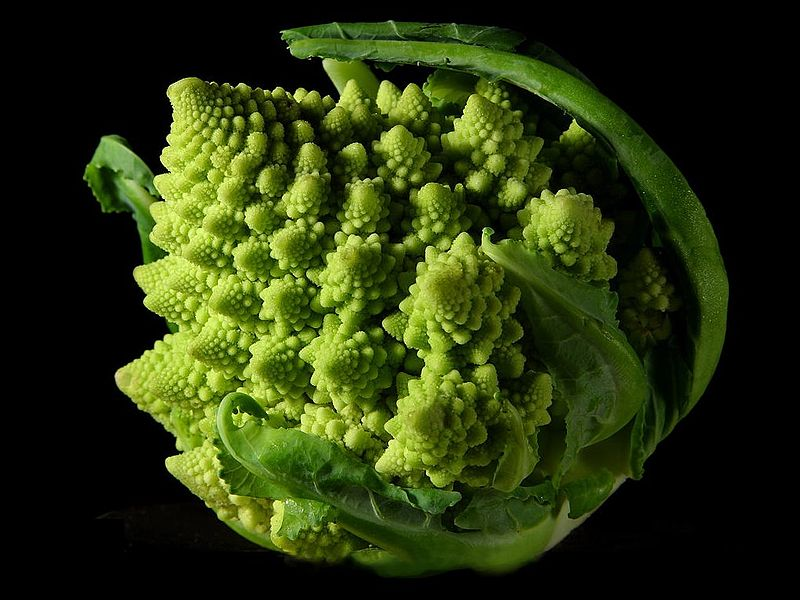
\includegraphics[width=0.3\textwidth]{broccoli}\footnote{By Jon Sullivan, \url{http://pdphoto.org/PictureDetail.php?mat=pdef&pg=8232}.}
      \end{center}
    \item Mathematics: The behaviour of finite sequences and series is connected with combinatorics (like we saw last
          week and will see next week), while the behaviour of infinite sequences and series is connected with calculus.
  \end{itemize}
\end{tcolorbox}
\end{center}

\clearpage
\subsection*{Questions}
[This is a sample Ministry of Education L2 assessment task for this standard.]

This assessment activity requires you to create a fractal and use sequences and series to investigate features of the shape. Features of fractals
include such things as length, area, number of items, volume.

Create your own fractal.
Include:
\begin{itemize}
  \item Details of how the fractal is created, i.e. the initial unit segment or shape, and how your fractals are formed, including diagrams.
  \item The values generated for at least three stages (after the initial stage) of the fractal for at least two of the features of the fractal.
  \item The totals for at least two features of the fractal for any given stage.
  \item Describe what will happen to the values and totals for each feature as the number of iterations increases.
  \item For your chosen features, will there be a point where the next iteration makes no significant difference to the feature? Describe the conditions
        under which this might happen.
\end{itemize}

The quality of your reasoning and how well you link this context to generalisations of arithmetic and geometric sequences will determine the
overall grade. Include calculations, diagrams or formulae, as appropriate. Clearly communicate your method using correct mathematical statements
where appropriate.

\end{document}
